\section{Valtorria}\label{valtorria}

Tags: Città Creatore: Davide, Lorenzo Ispirazione: Salerno

\section{Valtorria}\label{valtorria-1}

\begin{center}\rule{0.5\linewidth}{0.5pt}\end{center}

\begin{figure}
\centering
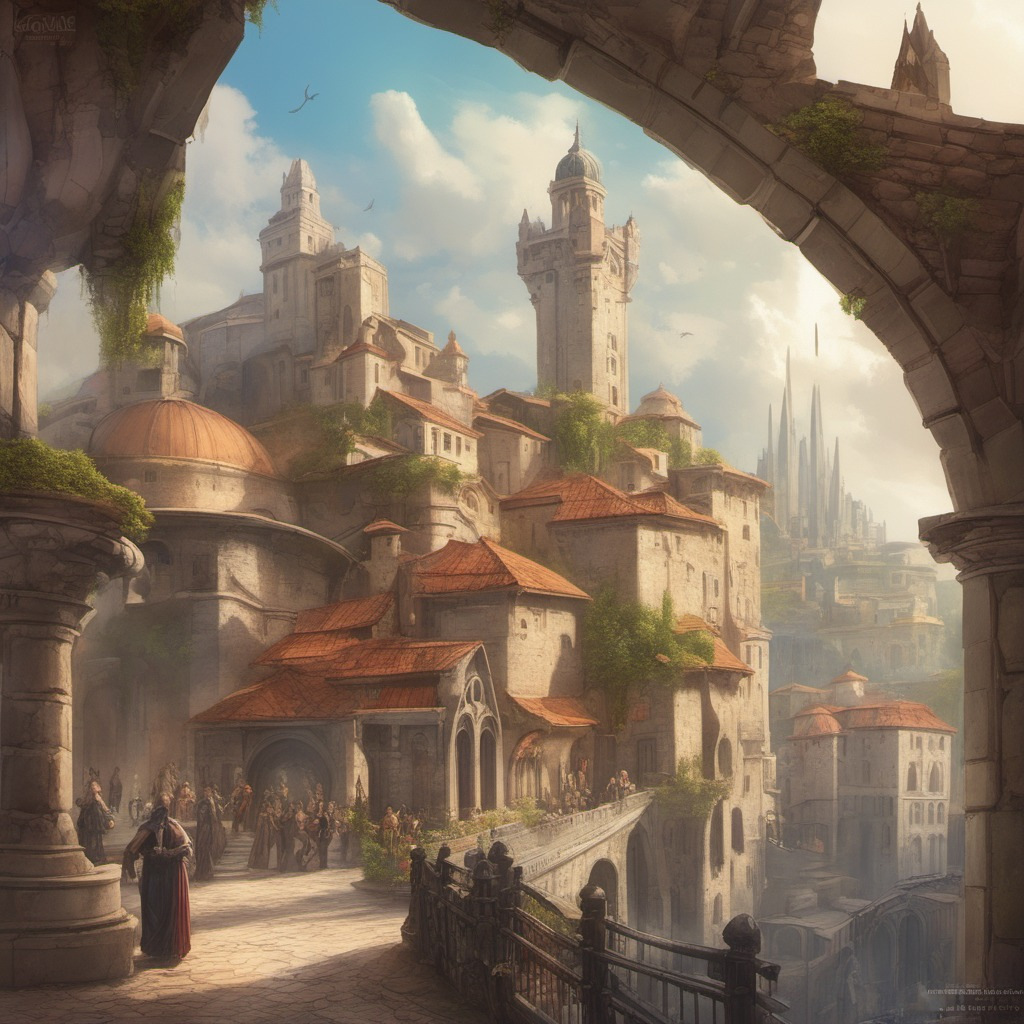
\includegraphics{WhatsApp_Image_2023-08-01_at_18.19.40.jpeg}
\caption{WhatsApp Image 2023-08-01 at 18.19.40.jpeg}
\end{figure}

Informazioni Generali

Tipo di Luogo: Città

Dimensioni:

Altitudine: 53m slm

Popolazione: 23000

Paese: Valtara

Luogo:

Alleata con: Cac Hanzaro

Attività: Cantiere navale

\begin{center}\rule{0.5\linewidth}{0.5pt}\end{center}

\subsection{1. Descrizione Generale}\label{descrizione-generale}

\begin{center}\rule{0.5\linewidth}{0.5pt}\end{center}

Valtorria è una affascinante e leggendaria città fantasy situata sulle
coste della regione di Valtara. La sua ricca storia risale a un'epoca
passata in cui fungeva da capitale di un potente impero che regnava su
tutta la regione di Valtara. Col passare del tempo, il suo legato è
rimasto vivo e, ancora oggi, è un tesoro prezioso di Valtara, rinomato
per le sue splendide luminarie.

\subsection{2. Storia}\label{storia}

\begin{center}\rule{0.5\linewidth}{0.5pt}\end{center}

Nell'antichità, Valtorria era il cuore di un potente impero,
abbracciando una cultura vibrante e una prosperità fiorente. Il dominio
dell'impero si estendeva per l'ampia estensione di Valtara, consolidando
la posizione di Valtorria come centro cruciale di arte, commercio e
conoscenza. La maestosa architettura della città, caratterizzata da
torri imponenti, palazzi intricati e monumenti sontuosi, testimoniava la
sua passata grandezza.

Guerre, carestie e lotte intestine minarono la stabilità dell'impero,
gettando un'ombra oscura sul suo dominio. Questi turbamenti portarono
alla perdita del controllo su molte regioni che un tempo dipendevano da
Valtorria, spezzando legami che erano stati forgiati attraverso
generazioni. Gradualmente, la città iniziò a sgretolarsi, perdendo il
suo prestigio e il suo splendore passati. Le strade una volta affollate
si svuotarono, i palazzi magnifici caddero in rovina, e l'antica gloria
si dissolse come sabbia nelle mani. Con il passare dei secoli, Valtorria
divenne un riflesso sbiadito del suo antico sé, un simbolo di ciò che
era stato e di ciò che poteva ancora diventare.

Nell'epoca attuale, Valtorria si erge come una città indipendente,
tuttavia, è influenzata dalle complesse dinamiche politiche che agiscono
nella regione, sia da città-stato che da regni circostanti. Alla guida
di questa affascinante città si trova il visionario leader Enzosor. La
sua dedizione costante è rivolta a riportare Valtorria alla sua antica
grandezza, preservando al contempo la sua rilevanza storica e
incoraggiando un futuro radioso. Mentre Valtorria si sforza di mantenere
la sua indipendenza e di riprendersi la sua gloria perduta, il ruolo di
Enzosor si rivela cruciale nel negoziare e mantenere un equilibrio
delicato con le forze politiche circostanti. Questa dinamica complessa
rende Valtorria un crogiolo di intrecci politici e culturali, una città
destinata a brillare nel panorama della regione di Valtara, con il suo
patrimonio culturale, la sua maestosità architettonica e la magia
intrinseca del Festival delle Luminarie a illuminare il cammino verso un
futuro ambizioso.

\subsection{3. Geografia}\label{geografia}

\begin{center}\rule{0.5\linewidth}{0.5pt}\end{center}

\subsubsection{3.1 Caratteristiche
Costiere}\label{caratteristiche-costiere}

\begin{center}\rule{0.5\linewidth}{0.5pt}\end{center}

Le coste di Valtorria presentano una morfologia variegata,
caratterizzata da ampie distese di sabbia dorata e basse scogliere.
Queste scogliere, grazie alla loro struttura, fungono da barriera
naturale contro l'erosione costiera, proteggendo il litorale dalle forze
dell'oceano. Le spiagge sabbiose offrono un ambiente accogliente per i
visitatori e la comunità locale, creando una sinergia tra l'uomo e il
mare. La presenza di una zona costiera relativamente bassa è stata un
fattore chiave nella crescita della città e nella sua dipendenza dal
mare come fonte di risorse, commercio e attività portuali.

\subsubsection{3.2 Caratteristiche
Montane}\label{caratteristiche-montane}

\begin{center}\rule{0.5\linewidth}{0.5pt}\end{center}

La peculiare disposizione geografica di Valtorria si manifesta nella
vicinanza tra la zona costiera e l'altopiano montuoso, poiché le
montagne si ergono a pochi chilometri dalla costa. Questa prossimità tra
l'ambiente marino e montano crea una transizione affascinante tra i due
paesaggi. Le imponenti montagne, caratterizzate da pendii scoscesi e
cime che si innalzano verso il cielo, offrono panorami mozzafiato sulla
città e sull'orizzonte marino. Questa stretta contiguità tra mare e
montagna crea un microclima unico, influenzando le condizioni
meteorologiche locali e arricchendo la biodiversità della regione.

\subsection{4. Demografia}\label{demografia}

\begin{center}\rule{0.5\linewidth}{0.5pt}\end{center}

La demografia di Valtorria è un affascinante e complesso quadro che
riflette il susseguirsi delle ere e degli eventi che hanno segnato la
storia della città. Situata nella regione di Valtara, questa città ha
subito notevoli mutamenti demografici, plasmando la sua popolazione in
modi sorprendenti.

\subsubsection{\texorpdfstring{4.1 \textbf{Popolazione
Attuale}}{4.1 Popolazione Attuale}}\label{popolazione-attuale}

\begin{center}\rule{0.5\linewidth}{0.5pt}\end{center}

Valtorria ospita attualmente una popolazione diversificata, composta
principalmente da discendenti dei cittadini che hanno scelto di rimanere
fedeli alla città durante i periodi tumultuosi della sua storia. La
popolazione attuale è stimata a {[}numero{]}, rendendo Valtorria una
comunità di dimensioni moderate.

\subsubsection{\texorpdfstring{4.2 \textbf{Gruppi
Etnici}}{4.2 Gruppi Etnici}}\label{gruppi-etnici}

\begin{center}\rule{0.5\linewidth}{0.5pt}\end{center}

La città di Valtorria è un melting pot di etnie e culture. Tra i gruppi
etnici più rappresentati troviamo {[}elenco di gruppi etnici{]}, ognuno
dei quali contribuisce alla ricchezza culturale della città. Questa
diversità etnica è una testimonianza delle influenze che hanno plasmato
Valtorria nel corso dei secoli.

\subsubsection{\texorpdfstring{4.3
\textbf{Lingue}}{4.3 Lingue}}\label{lingue}

\begin{center}\rule{0.5\linewidth}{0.5pt}\end{center}

La lingua predominante parlata a Valtorria è {[}lingua predominante{]},
ma a causa della diversificazione etnica, una varietà di lingue
minoritarie è diffusa tra le comunità di immigrati.

\subsubsection{\texorpdfstring{4.4 \textbf{Evoluzione
Storica}}{4.4 Evoluzione Storica}}\label{evoluzione-storica}

\begin{center}\rule{0.5\linewidth}{0.5pt}\end{center}

L'evoluzione demografica di Valtorria è stata caratterizzata da
cambiamenti significativi. Durante il periodo dell'impero, la città era
una folla vivace e cosmopolita, attirando persone da tutte le parti di
Valtara. Tuttavia, con la caduta dell'impero e i secoli di instabilità,
la popolazione diminuì drasticamente.

Negli anni recenti, Valtorria ha assistito a un modesto incremento
demografico, grazie agli sforzi del suo leader, Enzosor, di riportare la
città alla sua antica grandezza e attirare nuovi abitanti.

La demografia di Valtorria è una testimonianza della sua storia
travagliata e della sua capacità di adattarsi e prosperare nonostante le
avversità. La diversità etnica e culturale contribuisce alla ricchezza
della vita cittadina, creando una comunità vibrante e aperta al futuro.

\subsection{5. Economia}\label{economia}

\begin{center}\rule{0.5\linewidth}{0.5pt}\end{center}

L'economia di Valtorria è un riflesso della sua storia ricca e
variegata, con un'evoluzione che ha trasformato la città da un centro
economico imperiale a un'entità più autonoma e dinamica. Oggi, Valtorria
prospera grazie a un'economia diversificata che abbraccia diversi
settori chiave. Uno degli aspetti più distintivi dell'economia di
Valtorria è la presenza dei suoi grandi cantieri navali, che
costruiscono navi per una vasta gamma di scopi, tra cui militari,
commerciali e privati.

\subsubsection{\texorpdfstring{5.1 \textbf{Commercio e
Artigianato}}{5.1 Commercio e Artigianato}}\label{commercio-e-artigianato}

\begin{center}\rule{0.5\linewidth}{0.5pt}\end{center}

Valtorria è stata storicamente conosciuta per il suo ruolo centrale nel
commercio e nell'artigianato. La città, con le sue radici nel passato
imperiale, è un importante centro di produzione di beni artigianali di
alta qualità. Oggetti artistici, gioielli lavorati a mano e manufatti
magici sono alcune delle specialità artigianali di Valtorria. Il
commercio di questi prodotti alimenta la città e attrae mercanti e
acquirenti da tutto il continente.

\subsubsection{\texorpdfstring{5.2 \textbf{Agricoltura e
Alimentazione}}{5.2 Agricoltura e Alimentazione}}\label{agricoltura-e-alimentazione}

\begin{center}\rule{0.5\linewidth}{0.5pt}\end{center}

Le fertili terre circostanti Valtorria forniscono una varietà di
prodotti agricoli di alta qualità. Valtorria è rinomata per la
produzione di vini pregiati, prodotti lattiero-caseari e prelibatezze
gastronomiche. Il settore alimentare è in costante crescita, con
ristoranti, enoteche e mercati che soddisfano i palati dei cittadini e
dei visitatori.

\subsubsection{\texorpdfstring{5.3 \textbf{Cantieri Navali di
Valtorria}}{5.3 Cantieri Navali di Valtorria}}\label{cantieri-navali-di-valtorria}

\begin{center}\rule{0.5\linewidth}{0.5pt}\end{center}

I cantieri navali di Valtorria sono rinomati in tutto il continente per
la loro maestria nella costruzione navale. Questi cantieri producono
navi di alta qualità, che vengono vendute a nazioni vicine e lontane. La
loro specializzazione nella costruzione di navi militari, commerciali e
private ha contribuito in modo significativo all'economia della città.
Questa industria è stata una fonte di orgoglio per i cittadini di
Valtorria, che mantengono una lunga tradizione di maestria nella
costruzione navale.

\subsubsection{\texorpdfstring{5.4 \textbf{Commercio
Marittimo}}{5.4 Commercio Marittimo}}\label{commercio-marittimo}

\begin{center}\rule{0.5\linewidth}{0.5pt}\end{center}

L'industria navale di Valtorria ha stimolato anche lo sviluppo del
commercio marittimo. Le navi costruite nei cantieri di Valtorria solcano
gli oceani, portando merci preziose e stimolando lo scambio commerciale
tra la città e le altre regioni. Il porto di Valtorria è diventato
un'importante via di collegamento per il commercio marittimo e una
risorsa economica vitale per la città.

\subsubsection{\texorpdfstring{5.5 \textbf{Tecnologia e
Innovazione}}{5.5 Tecnologia e Innovazione}}\label{tecnologia-e-innovazione}

\begin{center}\rule{0.5\linewidth}{0.5pt}\end{center}

I cantieri navali di Valtorria non solo costruiscono navi di alta
qualità, ma sono anche un centro di innovazione tecnologica. Gli
artigiani locali lavorano costantemente per migliorare la progettazione
e la tecnologia navale, rimanendo all'avanguardia nel settore. Questa
continua ricerca di eccellenza ha contribuito a mantenere la reputazione
di Valtorria come un centro di eccellenza nella costruzione navale.

\subsubsection{\texorpdfstring{5.6 \textbf{Arte e
Cultura}}{5.6 Arte e Cultura}}\label{arte-e-cultura}

\begin{center}\rule{0.5\linewidth}{0.5pt}\end{center}

L'arte e la cultura giocano un ruolo cruciale nell'economia di
Valtorria. La città attrae artisti, musicisti, e scrittori, alimentando
un'industria culturale in espansione. Le opere d'arte, le esibizioni
teatrali e i festival culturali contribuiscono all'economia locale e
all'attrattiva turistica.

\subsubsection{\texorpdfstring{5.7
\textbf{Turismo}}{5.7 Turismo}}\label{turismo}

\begin{center}\rule{0.5\linewidth}{0.5pt}\end{center}

Valtorria è una meta turistica di grande successo, grazie alla sua
storia affascinante, alla magnifica architettura e ai festival
culturali. Il turismo gioca un ruolo essenziale nell'economia della
città, con alberghi, ristoranti, e attività turistiche che offrono
servizi di alta qualità ai visitatori.

\subsection{6. Cultura}\label{cultura}

\begin{center}\rule{0.5\linewidth}{0.5pt}\end{center}

\subsubsection{\texorpdfstring{6.1 \textbf{Festival delle
Luminarie}}{6.1 Festival delle Luminarie}}\label{festival-delle-luminarie}

\begin{center}\rule{0.5\linewidth}{0.5pt}\end{center}

Il Festival delle Luminarie è una delle tradizioni più celebrate di
Valtorria, una magnifica celebrazione annuale che richiama visitatori da
ogni angolo della regione di Valtara. Durante questo incantevole
spettacolo, la città si veste di una straordinaria esposizione di
decorazioni luminose. Innumerevoli lanterne intricate, che emanano un
bagliore etereo, adornano le strade e gli edifici, trasformando il cielo
notturno in un mare di stelle scintillanti. Questo festival non solo
simboleggia l'unità della regione, ma è anche un vivido ricordo della
gloriosa storia di Valtorria. Ogni anno, abili artigiani e artisti
provenienti da Valtorria e dalle città vicine investono la loro maestria
creativa nella realizzazione di queste luminarie, contribuendo a rendere
il festival un'esperienza indimenticabile per tutti coloro che vi
partecipano. Le luminarie sono opere d'arte luminose, frutto di
dedizione e passione, e catturano l'immaginazione di tutti coloro che le
ammirano, trasportandoli in un mondo di magia e meraviglia. Il Festival
delle Luminarie è un evento atteso con trepidazione da parte di ogni
abitante di Valtorria e un'opportunità per celebrare l'orgoglio e
l'identità culturale della città. Oltre a essere un'attrazione per i
visitatori, il festival rafforza anche i legami tra le diverse comunità
della regione di Valtara, unendole in un'atmosfera di gioia e
festeggiamenti. Le luci brillanti e le splendide forme delle luminarie
trasformano Valtorria in un regno di incanto, catturando i cuori di
coloro che si immergono in questa festa magica. Il Festival delle
Luminarie è un omaggio alla grandezza passata di Valtorria e un segno
luminoso di speranza per il suo futuro radioso. Ogni anno, mentre le
lanterne si accendono e il cielo si illumina, Valtorria risplende ancora
una volta nel suo antico splendore, invitando tutti a unirsi a questa
celebrazione straordinaria.

\subsection{7. Governo}\label{governo}

\begin{center}\rule{0.5\linewidth}{0.5pt}\end{center}

Valtara è governata da un sistema politico unico con caratteristiche di
oligogerontocrazia. Il Sindaco, scelto da un collegio di anziani saggi,
è il capo della città e dell'esercito, e viene eletto ogni sette anni
attraverso elezioni democratiche. La sua leadership militare garantisce
la sicurezza della città. Le autorità religiose del Tempio
dell'Equilibrio hanno un ruolo influente, guidando le decisioni etiche e
morali. Questa forma di governo riflette un equilibrio tra leadership,
sicurezza e spiritualità, contribuendo al benessere e alla stabilità di
Valtara, una prospera metropoli con una ricca diversità culturale.

\begin{figure}
\centering
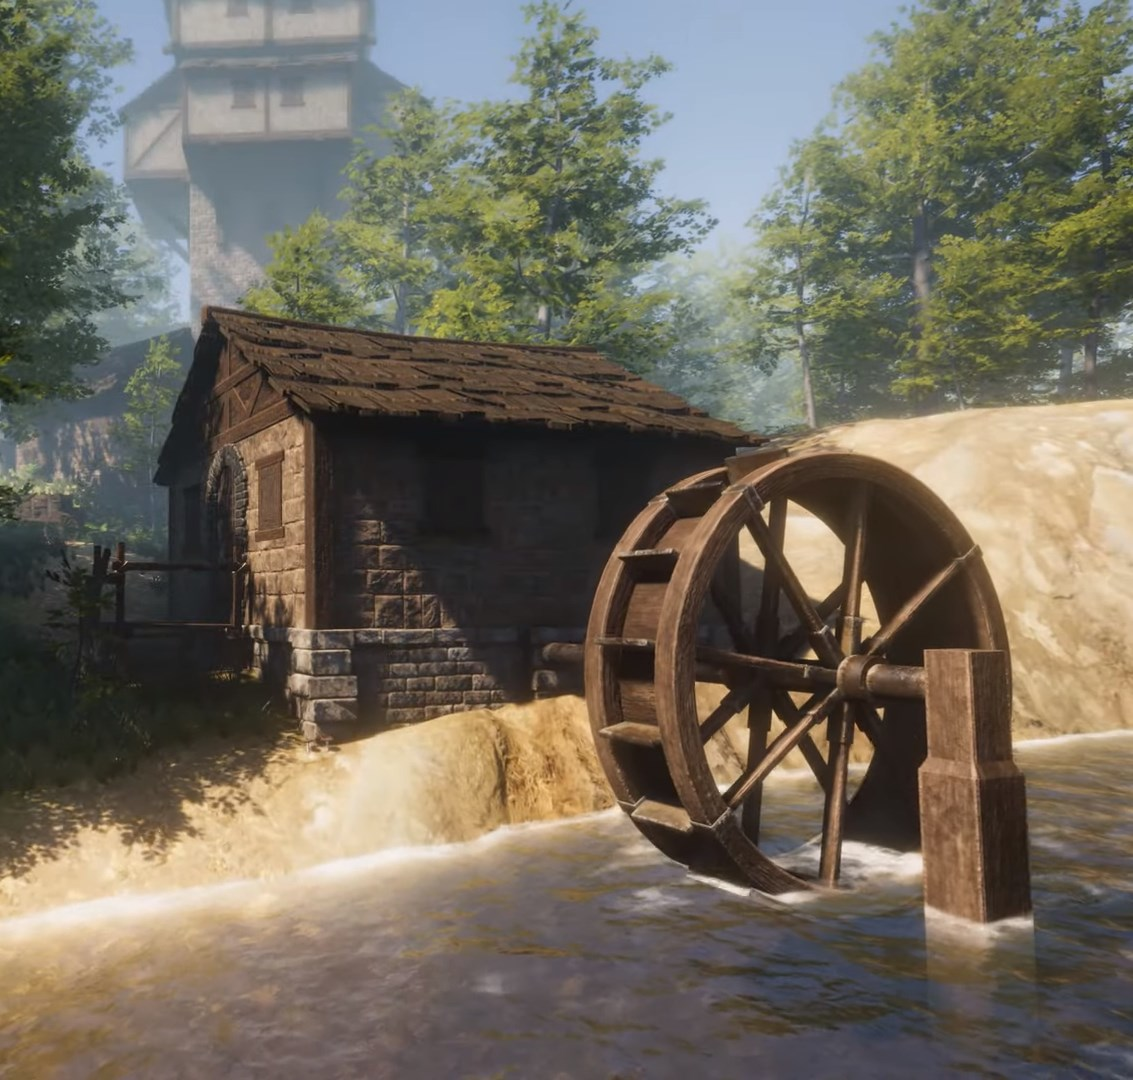
\includegraphics{chrome_0v22jZh2os.jpg}
\caption{chrome\_0v22jZh2os.jpg}
\end{figure}

\subsubsection{7.1 Consiglio degli Anziani e Consiglio dei
Rappresentanti}\label{consiglio-degli-anziani-e-consiglio-dei-rappresentanti}

\begin{center}\rule{0.5\linewidth}{0.5pt}\end{center}

Il Consiglio di Valtara è composto da un gruppo selezionato di anziani
saggi, noti come ``Collegio degli Anziani''. Questi membri sono scelti
per la loro saggezza, esperienza e competenza in diversi campi, tra cui
politica, giurisprudenza, economia e cultura. Il loro ruolo principale è
quello di fungere da consiglieri del Sindaco e di contribuire alla
formulazione delle politiche e delle decisioni che riguardano la città.
Il Consiglio dei Rappresentanti è invece l'organo legislativo di
Valtara, composto da membri eletti direttamente dalla popolazione
attraverso elezioni democratiche. Questi rappresentanti hanno il compito
di rappresentare gli interessi e le esigenze della comunità e di
proporre e approvare leggi e politiche che influenzano la vita di
Valtara. Il Consiglio è un organo consultivo che gioca un ruolo cruciale
nel governo di Valtara, fornendo una vasta gamma di competenze e
prospettive per guidare la città verso un futuro prospero e armonioso.
La sinergia tra il Collegio degli Anziani e il Consiglio dei
Rappresentanti assicura un governo equilibrato, inclusivo e
rappresentativo, con una governance partecipativa che tiene conto delle
esigenze e delle aspettative della popolazione di Valtara.

\subsection{8. Persone famose}\label{persone-famose}

\begin{center}\rule{0.5\linewidth}{0.5pt}\end{center}

\begin{itemize}
\tightlist
\item
  \href{Enzhosor\%20Ent\%20Ino\%20d098e258d48c4aaea0dccbf531c4688c.md}{Enzhosor
  Ent Ino}
\end{itemize}
